% Introduction

\chapter{Introduction} % Main chapter title

\label{chapter:introduction}

%----------------------------------------------------------------------------------------

% Define some commands to keep the formatting separated from the content 
\newcommand{\keyword}[1]{\textbf{#1}}
\newcommand{\tabhead}[1]{\textbf{#1}}
\newcommand{\code}[1]{\texttt{#1}}
\newcommand{\file}[1]{\texttt{\bfseries#1}}
\newcommand{\option}[1]{\texttt{\itshape#1}}

%----------------------------------------------------------------------------------------
\section{Background}
The accretion of \enquote{Smart technology} and \enquote{Industry 4.0} has led to some revolutionary scientific development in the field of software development and networking. As a consequence, new features like the backend gateway applications are introduced to interconnect the physical or human-operated systems to monitor the data over the Internet, adding more operation reliability. The term \ac{IoT} has bridged the gap between the hardware and software worlds. A majority of embedded products in the market has brought in the concept of compact design with minimal cost. In the last few decades, there has been a huge demand of cost effective Embedded hardware and \ac{SoC} and it is continue to rise exponentially with each passing year. 

The major focus area of an embedded design from the software platform perspective is to choose an OS where one can build applications or libraries very easily and Linux seems as the preferable choice. On top of that, major Linux distributions uses the OpenEmbedded framework to build custom Linux distribution.  It provides with the set of development tools, recipes, and configurations to support th build process. The OpenEmbedded build system utilizes "Poky", a Yocto project distribution. As the Yocto Project documentation defines, “It contains the OpenEmbedded Build System (BitBake and OpenEmbedded Core) as well as a set of metadata to get started with building custom distribution.”~\parencite{Reference2} In general, BitBake is the task executor which handles the build process. According to organization requirement needs, certain applications or packages are externally integrated into the build system. These applications are designed and developed through a software release lifecycle. One such example is \keyword{\ac{REST} \ac{API}}, or REST API, application to transfer state of point resources in the form of \ac{JSON} to the endpoint via HTTP. However, with each software release, there is a necessity to test these applications or software via manual, data-driven, acceptance testing with test frameworks like Robot. This paves way for DevOps, continuous integration and deployment which aids to greater functionalities to generate test reports, trigger email notification, and even upload to cloud artifactory (JFrog, GitHub).  Lastly, BitBake can also process the test reports at the event of build launch. In case, the test suite is not present, the quality of the software is compromised. Therefore, it is very critical for a project, that the test suite should be present and cover all the feature implementations before its final release. The next few chapters will present more detailed overview and practical scenarios why it is vital to have each application test reports in the build directory of the Linux distribution and discuss on ways to implement it via BitBake class files. 
%----------------------------------------------------------------------------------------

\section{Work Environment}

The master thesis work was conducted under the guidance of Mr. Nico Mueller and Dr. Martin Buschbeck from \emph{Bosch Thermotechnik GmbH}, department of \emph{TT-RHC/XAT}. The company, situated in Lollar, is a wholly-owned subdivision of \emph{Robert Bosch GmbH}.
The world-renowned company is prominent in the field of \enquote{heating and energy efficient technologies}. The company's product portfolio includes \textsc{HVAC} (heating,ventilation, and air conditioning) systems for instance hot-water solutions and water-heating solutions, boilers. \emph{Bosch Thermotechnik GmbH} produces more than 20 plants worldwide with more than 14,000 employees over 23 locations. 



In addition, the department \emph{TT-RHC/XAT} focuses on feature implementation of the IT backend gateways via mobile device, laptop to connect to its business models. For example, the gateway system to control a heating device via smartphone, providing strongest security in parallel. The team is also working towards enhancements and implementation of new embedded products. Products like the \emph{ Internet-Gateway MB LAN2} can connect to the heating system via \textsc{Bosch HomeCom Easy App} mobile application. It is also easy to install on the router via LAN cable. The gateway \emph{Logamatic web KM300} has significant advantages as well as it connects the heating system via the Internet. This leads to location-independent operation and monitoring. This thesis work also focuses on one such embedded product for car charging solutions.

%----------------------------------------------------------------------------------------

\section{Problem Statement}

The prerequisite of building a custom Linux distribution with the Yocto Project is a build framework. The Yocto project uses the OpenEmbedded as the build framework which in turn use Poky, a \keyword{reference distribution} with necessary Yocto project tools to set up the build environment. The build environment contains metadata, which consists of configuration files, recipes, classes, etc.  The metadata is parsed by the OpenEmbedded build system while launching the build. Consequently, metadata has many pre-installed recipes and few additional recipes for software components that are targeted for a specific project depending on the requirements of the department and the customer. For example, applications such as the \ac{REST} \ac{API}, web configuration are among the few target software components that these additional recipes hold for building a custom Yocto image. In a potential \ac{ALM}, these applications are designed, developed, and tested thoroughly within each release. To further automate the process, continuous integration and continuous deployment are configured as a part of \ac{SDLC}. A \ac{CI} tool is more like an orchestrator, connected to the Version Control system (Git) ~\parencite{pathania2017learning} to automate the application build, testing and deploy phase. The thesis work was also implemented out on a Jenkins server licensed by \emph{Bosch}. In the test phase of the \ac{ALM}, the stakeholders\footnote{Stakeholders: Development Team, Testers, Customers, Project Managers} have the possibility to refer to the application test report that are guidelines for passed or failed features or flaw in the application.

As a part of the \keyword{Product release cycle}, the build process is automated with the Jenkins pipeline containing pre and post build actions. It requires a build repository with all the manifest files that holds the metadata information. At the build setup/development stage, BitBake process layers, metadata, parses application recipes files and a Yocto image is created, followed by image testing and then the final deployment to an artifactory. The image is then ready to be delivered and mounted on an embedded product.


At the delivery phase of the release, there is no provision for the stakeholders to refer to all the application test reports under one directory. They either need to refer to the application test reports performed at the \ac{ALM} phase outside the Yocto level or traditionally run the application test suite which is challenging. The best practice is to somehow link or fetch these application test reports into the Yocto build directory during build launch. The work aims to find a potential solution of \keyword {Software Integration} at the Yocto level and bring all these application test reports under one single directory along with Linux \ac{OS} images, Licenses, etc. Refer to the architectural overview of the problem statement ( See Figure \ref{fig:Architectural summary of the Problem Statement}) 



\begin{figure}
\centering
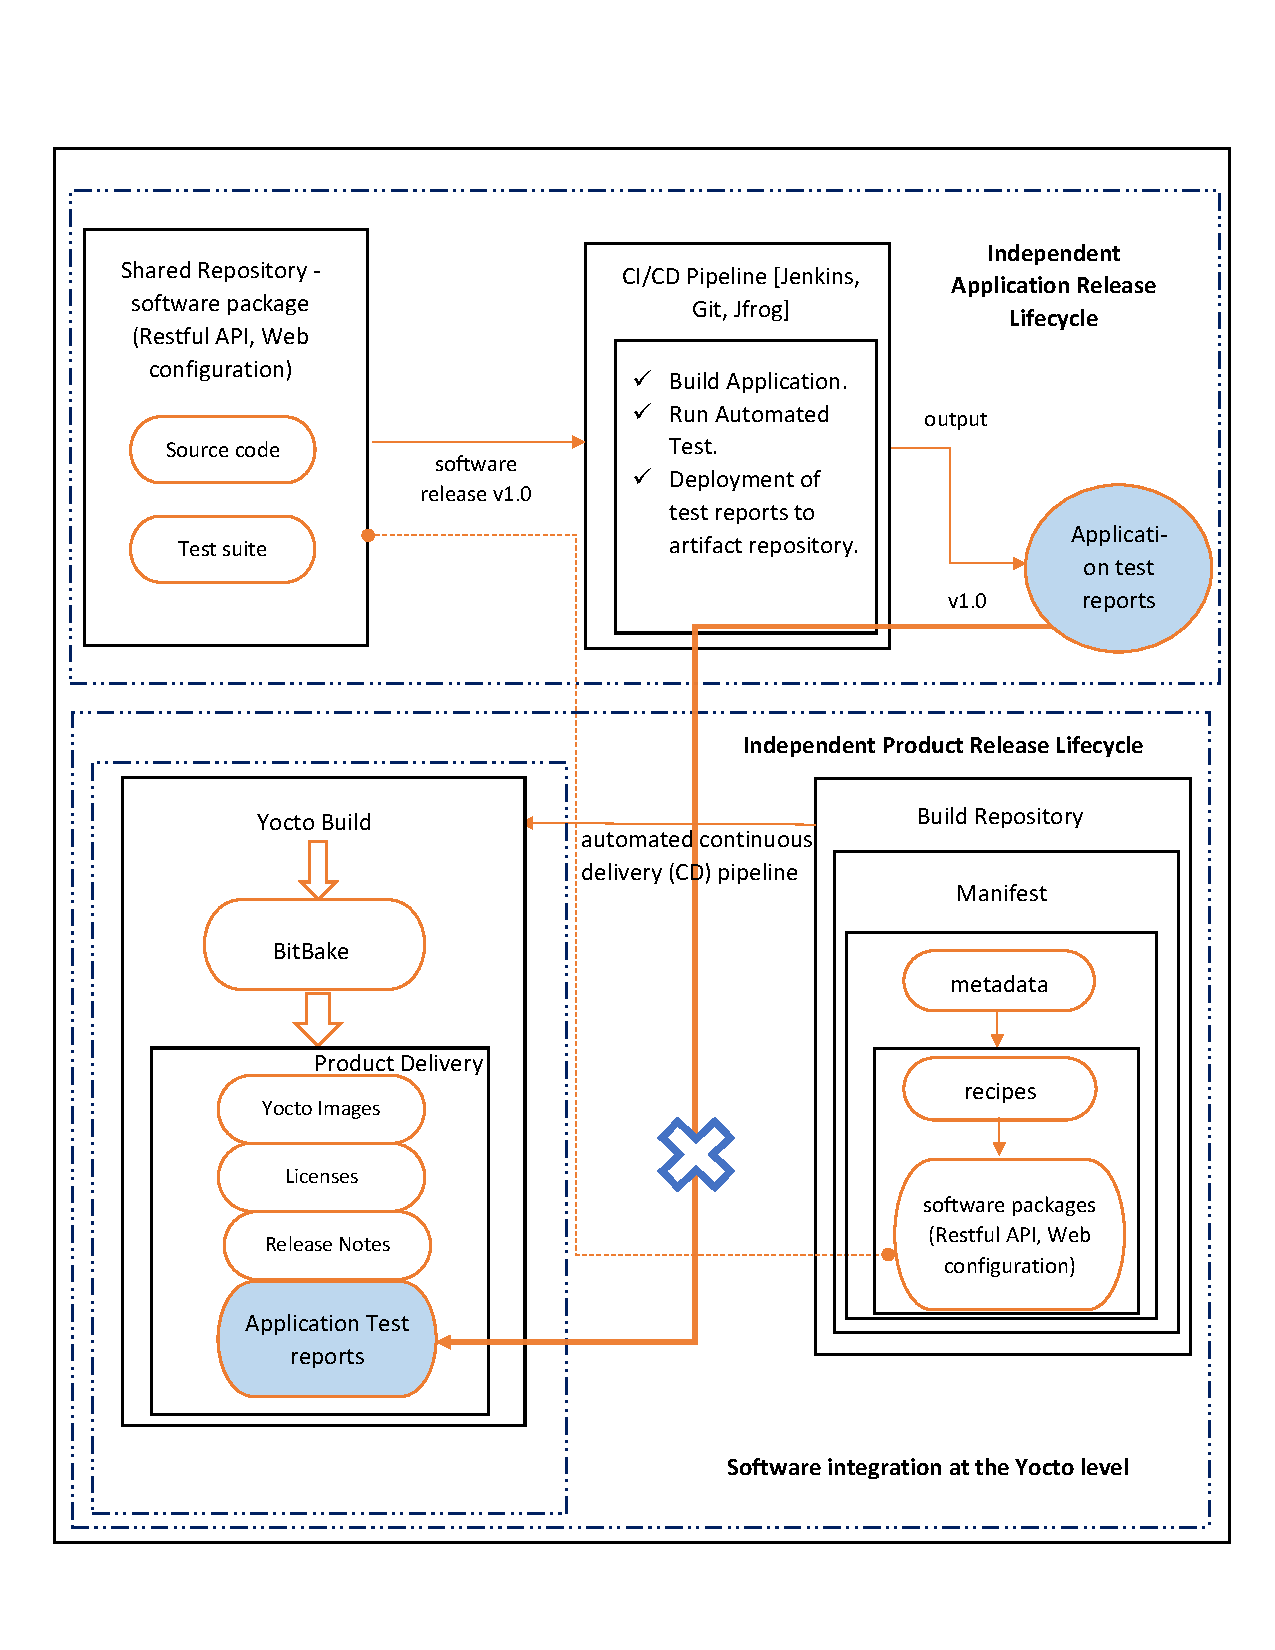
\includegraphics[scale=0.7]{figures/ThesisYocto.pdf}
\caption[Architectural summary of the Problem Statement]{Architectural summary of the Problem Statement.}
\label{fig:Architectural summary of the Problem Statement}
\end{figure}


%----------------------------------------------------------------------------------------
\newpage
\section{Objectives}

The aim of the thesis work is to first address the key concerning area by identifying and analyzing the concept of Software Integration and Delivery at a Product level. Thereafter, the understanding of the existing software development architecture within the department is necessary to recognize the current shortcomings and how this research can enhance and improve the Software and Product release lifecycle. The present study researches the implemented work in the area of custom embedded Linux distribution with the Yocto project. Tools and products, used for the implementation purpose in this thesis are all licensed by \emph{Bosch Thermotechnik GmbH}.

\vspace{0.2cm}
The paper highlights out few following questions and strive for the best  solution approach.  
\vspace{0.2cm}
\begin{itemize}

\item \emph{What is the concept of Software Integration and Software Delivery ?}
\item \emph{What are the deliverables of the target product ?}
\item \emph{How to integrate the product deliverables into the delivery package at the Yocto level ?}
\item \emph{How does the thesis work improves the Product release lifecycle ?}
\end{itemize}

%----------------------------------------------------------------------------------------

\section{Thesis Outline}

Major companies have welcomed the modern approaches of application development by driving automation into projects. The commencement of DevOps practice has brought in a significant impact on development speed and time to market for a product. The aim of the work is to make use of \ac{CI}, \ac{CD} pipeline to test various software applications and analyze test reports. Furthermore, these test reports are packaged into an artifact, which can then be fetched into the Yocto build host with the help of BitBake and Yocto classes. The work is carried out only on internal applications and products owned by the department. The thesis is organized into the following chapters:  
\begin{itemize}
\item \keyword{Chapter 1} - The chapter reflects the general terms used in the research paper quite often and also in areas of application testing phase with a spotlight on terms such as test automation, continuous integration and deployment pipeline, containerization. An overview of the embedded Linux distribution with the Yocto Project is also mentioned here with focus on class files (.bbclass) and recipe.

\item \keyword{Chapter 2} - Major portion of the research work including the efforts to run the application test suites and uploading the same to an artifact will be included here. Concurrently, the chapter analyzes on the implementation of the class file and other changes made to the recipe. The research outlines the development of a custom class file that extends the BitBake fetch module to obtain the automated test reports from a source path and unpack to the deploy directory in the build system. 

\item  \keyword{Chapter 3} - 

\item \keyword{Chapter 4} - This chapter summarize the thesis and draw possible conclusion and future work.

\end{itemize}



%----------------------------------------------------------------------------------------
\section{State of the art}

\clearpage\null\thispagestyle{empty}